\ExerciseChapter{聚类分析}

\label{chapter:3}

\section{往年题}

\par\addvspace{6pt}\noindent\begin{minipage}{\linewidth}

\subsection{单项选择题}

\Question{M15-5}{聚类分析的条件}

关于聚类分析，错误的是：


\begin{choices}

\item 系统聚类即层次聚类。

\item 样本量很大时可考虑快速聚类。

\item 必须预先指定层次聚类的类别数。

\item Q型与R型聚类都需要定义距离或相似性。

\item 类平均法和Ward法都会受到极端值影响。

\end{choices}

\end{minipage}\par\vspace{4pt}

\par\addvspace{6pt}\noindent\begin{minipage}{\linewidth}

\Question{M17-5}{聚类结果与算法}

关于聚类分析，正确的是：


\begin{choices}

\item 需要已经明确分类的训练样本。

\item 对变量的聚类分为系统聚类和快速聚类。

\item 不同聚类方法可能得到很不相同的结果。

\item 样本量超过100时，个体聚类应一律使用层次聚类。

\item 要求聚类变量服从多元正态。

\end{choices}

\end{minipage}\par\vspace{4pt}

\par\addvspace{6pt}\noindent\begin{minipage}{\linewidth}

\Question{M21-5}{聚类方法与分布}

关于聚类分析，正确的是：


\begin{choices}

\item 需要已有分类的训练样本。

\item 对变量聚类分为系统聚类和快速聚类。

\item 不同聚类方法可能得到很不相同的结果。

\item 样本量超过100时，个体聚类应一律用层次聚类。

\item 聚类对变量分布无要求，但马氏距离要求变量正态。

\end{choices}

\end{minipage}\par\vspace{4pt}

\par\addvspace{6pt}\noindent\begin{minipage}{\linewidth}

\Question{N19-9}{K-means的目标}

通常K-means聚类最小化的是：


\begin{choices}

\item 类内欧氏平方距离总和。

\item 类间距离总和。

\item 所有样本的最大相关系数。

\item 类别先验概率的乘积。

\item 标签的错误率，且必须有训练标签。

\end{choices}

\end{minipage}\par\vspace{4pt}

\par\addvspace{6pt}\noindent\begin{minipage}{\linewidth}

\Question{N21-15}{Jaccard忽略什么}

二元属性中，Jaccard相似性不把哪一项计作相似证据？


\begin{choices}

\item 共同阳性。

\item 共同阴性。

\item 单侧阳性。

\item 所有阳性。

\item 所有不一致。

\end{choices}

\end{minipage}\par\vspace{4pt}

\par\addvspace{6pt}\noindent\begin{minipage}{\linewidth}

\Question{N21-16}{随机初值与复现}

为了复现使用随机初值的K-means结果，最应同时记录：


\begin{choices}

\item 只记录变量数。

\item 随机种子、标准化规则、k、重复初值次数与算法版本。

\item 只记录最终标签的顺序。

\item 只记录样本均值。

\item 只记录显著性水平。

\end{choices}

\end{minipage}\par\vspace{4pt}

\par\addvspace{6pt}\noindent\begin{minipage}{\linewidth}

\Question{N21-17}{代表变量的选择方向}

以类内平均平方相关作为代表性：\(v_j=\sum_{l\ne j}r_{jl}^2/(m-1)\)。应优先选择：


\begin{choices}

\item \(v_j\)最大者。

\item \(v_j\)最小者。

\item 变量名最短者。

\item 第1列且无需计算。

\item 方差最大的变量且不考虑相关性。

\end{choices}

\end{minipage}\par\vspace{4pt}

\par\addvspace{6pt}\noindent\begin{minipage}{\linewidth}

\subsection{简答题}

\Question{CS20}{Jaccard与简单匹配距离}

Jaccard距离和简单匹配距离有何区别？何时适用Jaccard距离？


\worklines{3}

\end{minipage}\par\vspace{4pt}

\subsection{计算与分析题}

\Question{CSPORT}{运动生理数据的两种聚类输出}

表1---3为运动生理实验数据的统计分析结果。

\begin{enumerate}
\def\labelenumi{\arabic{enumi}.}
\tightlist
\item
  表1属于何种分析？
\item
  把表1的对象分为4类，写出分类结果。
\item
  表2属于何种分析？
\item
  根据表2---3，运动水平高者在哪一类？
\item
  列出最无分类价值的两个变量。
\end{enumerate}

表1：

\begin{center}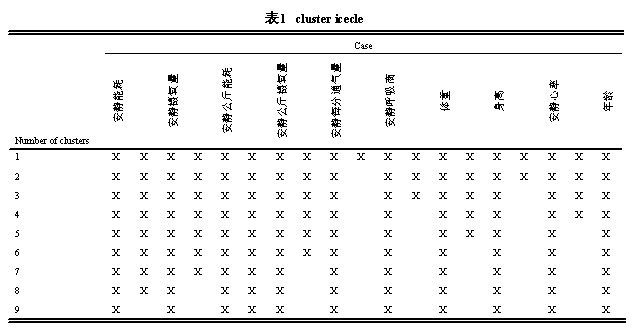
\includegraphics[width=\linewidth]{assets/sport_icicle.png}\end{center}

表2：最终分类中心。

\begin{center}\small\setlength{\tabcolsep}{4pt}\renewcommand{\arraystretch}{1.18}\begin{tabular}{@{}lrrrr@{}}
\toprule
指标 & 第1类 & 第2类 & 第3类 & 第4类 \\
\midrule

年龄 & 33 & 31 & 28 & 36 \\
身高 & 167 & 172 & 176 & 171 \\
体重 & 62 & 75 & 69 & 66 \\
安静心率 & 75 & 76 & 76 & 75 \\
安静每分通气量 & 8.5 & 11.2 & 13.4 & 10.0 \\
安静公斤摄氧量 & 4.4 & 5.8 & 6.8 & 5.0 \\
安静摄氧量 & 0.269 & 0.386 & 0.464 & 0.326 \\
安静呼吸商 & 0.86 & 0.83 & 0.84 & 0.85 \\
安静能耗 & 1882 & 2686 & 3313 & 2278 \\
安静公斤能耗 & 31 & 40 & 47 & 35 \\
\bottomrule\end{tabular}\end{center}

\begin{center}\small\setlength{\tabcolsep}{4pt}\renewcommand{\arraystretch}{1.18}\begin{tabular}{@{}lr@{}}
\toprule
分类 & 样本数 \\
\midrule

1 & 78 \\
2 & 67 \\
3 & 14 \\
4 & 97 \\
有效 & 256 \\
缺失 & 34 \\
\bottomrule\end{tabular}\end{center}


\worklines{3}

\par\addvspace{6pt}\noindent\begin{minipage}{\linewidth}

\Question{C19}{体质数据：Ward变量聚类与代表变量}

对体质数据进行变量聚类分析。共20分。

\begin{enumerate}
\def\labelenumi{\arabic{enumi}.}
\tightlist
\item
  用Ward法把变量分为5类，写出分类结果。
\item
  按一定统计规则，在``往返跑''所在类别中选择最有代表性的变量。
\item
  给出第2问的R代码，并解释变量及步骤含义。
\end{enumerate}

体质数据含脉搏、血压、肺活量、身高、体重、胸腰臀围、台阶指数、握力、背力、体前屈、纵跳、单脚站立、往返跑、反应时与俯卧撑等18项。


\worklines{3}

\end{minipage}\par\vspace{4pt}

\par\addvspace{6pt}\noindent\begin{minipage}{\linewidth}

\Question{C20}{夹角余弦与Ward变量聚类}

对体质数据的收缩压、舒张压、身高、体重、握力、背力、腰围、胸围、臀围、台阶指数、脉搏、往返跑12个变量聚类，指定相似性为夹角余弦，聚类方法为Ward法。共20分。

\begin{enumerate}
\def\labelenumi{\arabic{enumi}.}
\tightlist
\item
  给出冰柱图。（6分）
\item
  分为4类时，写出分类结果。（6分）
\item
  在变量数最多的类别中选择一个代表变量：常用选择方法有哪些？若按统计代表性最佳原则，报告计算结果和选择。（3+5分）
\end{enumerate}


\worklines{3}

\end{minipage}\par\vspace{4pt}

\par\addvspace{6pt}\noindent\begin{minipage}{\linewidth}

\Question{C21}{耳形数据：标准化与非标准化K-means}

使用ear数据做快速聚类，以EC、EK、EZ、EI、AI为变量，随机选4个初始中心，重复50次；按EC中心的升序将类别命名为1---4类。

\begin{enumerate}
\def\labelenumi{\arabic{enumi}.}
\tightlist
\item
  给出标准化聚类后第2类中心（还原到原量纲）。
\item
  给出非标准化聚类后第2类中心；另一回忆版本写``第3类''，请一并计算。
\item
  对EC=5、EK=2、EZ=2、EI=40、AI=50的待分类对象，用标准化聚类所获分类的类内协方差，列出到4类中心的马氏距离（取整数部分）和所属类别。
\end{enumerate}

指数定义：EI=100EK/EC，AI=100EZ/EK。


\worklines{3}

\end{minipage}\par\vspace{4pt}

\clearpage\section{补充练习}

本节为配合正文新编的补充练习。除注明沿用正文例题外，数值与研究摘要均为教学设定。题型与作答方式沿用本章往年题，解析见章末。

\par\addvspace{6pt}\noindent\begin{minipage}{\linewidth}

\subsection{单项选择题}

\Question{SUP-C1}{有序变量的距离}

两项有序指标分别有4级和5级，均按1开始编码。样品A的记录为 \((2,5)\)，样品B为 \((4,1)\)。按正文规定，对每项指标用其完整等级数 \(m\) 作 \(y=(x-1)/(m-1)\) 变换，再计算欧氏距离。两样品距离为：


\begin{choices}

\item \(\sqrt{20}\)。

\item \(\sqrt{5}/2\)。

\item \(2/3\)。

\item \(\sqrt{13}/3\)。

\item \(5/3\)。

\end{choices}

\end{minipage}\par\vspace{4pt}

\par\addvspace{6pt}\noindent\begin{minipage}{\linewidth}

\Question{SUP-C2}{负相关变量在R型聚类中的距离}

对指标作R型聚类。\(r_{AB}=-0.90\)，\(r_{AC}=0.50\)。研究者明确采用正文中的距离 \(d_{st}=\sqrt{1-r_{st}^2}\)。下列正确的是：


\begin{choices}

\item A与B的距离更小，该变换把较强的负相关也作为较强联系。

\item A与C的距离更小，因为负相关必定代表不相似。

\item A与B的距离为1.90。

\item A与B的距离为0.10。

\item 改用 \(d_{st}=1-r_{st}\) 后，两组距离的大小关系必定不变。

\end{choices}

\end{minipage}\par\vspace{4pt}

\par\addvspace{6pt}\noindent\begin{minipage}{\linewidth}

\subsection{简答题}

\Question{SUP-C3}{标准化欧氏距离与马氏距离}

研究者先将体重、胸围等指标作Z变换，再计算欧氏距离，并称：``标准化已经消除了量纲和变量相关性的影响，所以所得距离就是马氏距离。''请判断并说明理由。若改为对这些指标作R型聚类，中心化后的夹角余弦又与哪个统计量相同？


\worklines{3}

\end{minipage}\par\vspace{4pt}

\par\addvspace{6pt}\noindent\begin{minipage}{\linewidth}

\subsection{计算与分析题}

\Question{SUP-C4}{类间距离更新与两类划分}

4个样品在同一数值指标上的取值为 \(A=0\)、\(B=1\)、\(C=3\)、\(D=5.2\)，无需标准化。采用欧氏距离作凝聚型系统聚类，分别使用最短距离法、最长距离法和类平均法。这里类平均法指两类间所有样品对距离的算术平均。共15分。

\begin{enumerate}
\def\labelenumi{\arabic{enumi}.}
\tightlist
\item
  写出第一步合并的两个样品。（2分）
\item
  对第一步形成的新类，分别按三种方法计算它到其余两个样品的类间距离。（6分）
\item
  写出三种方法各自保留两类时的成员，并说明为何结果可能不同。（5分）
\item
  本题属于Q型还是R型聚类？（2分）
\end{enumerate}


\worklines{3}

\end{minipage}\par\vspace{4pt}

\par\addvspace{6pt}\noindent\begin{minipage}{\linewidth}

\Question{SUP-C5}{K-means收敛与类内平方和}

4个样品有两个尺度可比的数值指标，坐标分别为 \(A=(0,0)\)、\(B=(0,2)\)、\(C=(4,0)\)、\(D=(4,2)\)，本题不再标准化。取 \(k=2\)，用平方欧氏距离分配，每轮以类内均值更新中心。初始中心为 \(A\)、\(B\)。共15分。

\begin{enumerate}
\def\labelenumi{\arabic{enumi}.}
\tightlist
\item
  写出第一轮分配、更新后的两个中心，并判断下一轮分配是否变化。（5分）
\item
  计算该结果的类内平方和 \(W\)、总平方和 \(T\)、类间平方和 \(B_{\rm SS}\) 及 \(B_{\rm SS}/T\)。（5分）
\item
  若换用初始中心 \((0,1)\)、\((4,1)\)，求收敛后的 \(W\)，与前一结果比较。能否由``分配不再变化''认定已经找到全局最优？正文建议怎样降低初值影响？（5分）
\end{enumerate}


\worklines{3}

\end{minipage}\par\vspace{4pt}
\clearpage\section{习题解析}

\begin{keyidea}[核对方式]按题号核对。补写题目、原稿歧义及复算约定列在对应解析中。\end{keyidea}

\Answer{M15-5}{聚类分析的条件}

\textbf{答案：C。}

层次聚类先形成整个层次结构，再按所需类别数或切割高度划分；K-means等快速聚类通常需事先给定k。大样本的算法选择还取决于规模、距离和计算成本，不应把某个固定样本量当硬阈值。


\Answer{M17-5}{聚类结果与算法}

\textbf{答案：C。}

聚类是无监督分析，结果依赖变量、预处理、相似性及连接算法。常规距离聚类没有通用正态性要求；基于概率模型的聚类则需要相应模型假设。


\Answer{M21-5}{聚类方法与分布}

\textbf{答案：C。}

普通距离聚类无需通用正态假定；E的后半句错误，马氏距离作为度量不要求正态，使用其卡方分布进行推断才需要相应条件。回忆稿缺C/D，参考答案稿提供了完整内容。


\Answer{N19-9}{K-means的目标}

\textbf{答案：A。}

K-means交替更新分配与均值中心，以类内平方和为目标，可能得到局部最优。


\textbf{补写说明。} 2019卷该部分仅有总题数和部分回忆，整题内容未记录。本题为按课程知识点新编的补充练习，不是恢复的往年原题；编号只用于本包覆盖核对。


\Answer{N21-15}{Jaccard忽略什么}

\textbf{答案：B。}

Jaccard将共同阴性从分母和相似分子中排除，适合共同缺失缺乏含义的属性。


\textbf{补写说明。} 2021卷该部分仅有总题数和部分回忆，整题内容未记录。本题为按课程知识点新编的补充练习，不是恢复的往年原题；编号只用于本包覆盖核对。


\Answer{N21-16}{随机初值与复现}

\textbf{答案：B。}

随机起点、预处理和算法实现均会影响局部解；类别数字本身还可任意重新编号。


\textbf{补写说明。} 2021卷该部分仅有总题数和部分回忆，整题内容未记录。本题为按课程知识点新编的补充练习，不是恢复的往年原题；编号只用于本包覆盖核对。


\Answer{N21-17}{代表变量的选择方向}

\textbf{答案：A。}

该指标度量该变量与同类其余变量的平均联系强度；如果全部很小，还应质疑该类能否被单变量代表。


\textbf{补写说明。} 2021卷该部分仅有总题数和部分回忆，整题内容未记录。本题为按课程知识点新编的补充练习，不是恢复的往年原题；编号只用于本包覆盖核对。


\Answer{CS20}{Jaccard与简单匹配距离}

对二元变量，令 \(a\) 为共同阳性数，\(d\) 为共同阴性数，\(b+c\) 为不一致数： \[d_{\rm SM}=\frac{b+c}{a+b+c+d},\qquad d_J=\frac{b+c}{a+b+c}.\] 简单匹配把共同阴性也作为相似证据；Jaccard不计共同阴性。后者适用于``共同出现''有意义、共同缺失不足以说明相似的属性，如罕见特征或物种存在。并非只要阳性率不均衡就一定使用Jaccard；\(a+b+c=0\) 时需约定空集合处理。


\Answer{CSPORT}{运动生理数据的两种聚类输出}

表1是\textbf{变量的层次聚类冰柱图}，不是对个体的聚类。切为4组：

\begin{enumerate}
\def\labelenumi{\arabic{enumi}.}
\tightlist
\item
  安静能耗、安静摄氧量、安静公斤能耗、安静公斤摄氧量、安静每分通气量。
\item
  安静呼吸商。
\item
  体重、身高。
\item
  安静心率、年龄。
\end{enumerate}

表2是\textbf{个体快速聚类的最终中心}。按题目原解释，第三类年轻、体格和摄氧相关指标较高，判作运动水平高者，人数14。但仅凭安静代谢指标不能代替严格运动能力测量，应限定为本题表格的相对解释。

安静心率和安静呼吸商在四类中心间差别很小，按本表描述最缺乏分类价值；若需严格判定，还应结合组内变异及变量尺度，不能只比较不同量纲变量的绝对极差。


\Answer{C19}{体质数据：Ward变量聚类与代表变量}

沿用原参考解的相似性变换 \(d_{ij}=\sqrt{1-r_{ij}^2}\) 与 \texttt{ward.D2}，同课程体质数据复算分为：

\begin{itemize}
\tightlist
\item
  脉搏、台阶指数、体前屈、纵跳、单脚站立、往返跑、反应时、俯卧撑。
\item
  收缩压、舒张压。
\item
  肺活量、身高。
\item
  体重、胸围、腰围、臀围。
\item
  握力、背力。
\end{itemize}

类别编号和叶序可不同，成员集合才是核对重点。定义类内代表性 \(v_j=\sum_{l\ne j}r_{jl}^2/(m-1)\)，取最大者。往返跑所在类各值：

\begin{center}\small\setlength{\tabcolsep}{4pt}\renewcommand{\arraystretch}{1.18}\begin{tabular}{@{}lr@{}}
\toprule
变量 & 平均平方相关 \\
\midrule

wfp & 0.04985 \\
zt & 0.04269 \\
fwc & 0.03007 \\
fys & 0.02388 \\
djzl & 0.01996 \\
mb & 0.01275 \\
tjzs & 0.00852 \\
tqq & 0.00840 \\
\bottomrule\end{tabular}\end{center}

故选 \textbf{往返跑} 本身（约0.04985），但该类整体相关性偏弱，代表性有限。

\begin{verbatim}
members <- names(cluster)[cluster == cluster['wfp']]
R <- cor(data[, members])
v <- (colSums(R^2) - 1) / (length(members) - 1)
names(which.max(v))
\end{verbatim}

\texttt{members}为该类变量名；\texttt{R}为其相关阵；去掉对角线自相关1后取平均平方相关。原代码循环始终用了同一列并使用 \texttt{which.min}，不能据此选择最大代表性变量。

所用距离可理解为忽略相关符号的投影差异；若改用其他距离/标准化方式，须说明，分类未必相同。


\Answer{C20}{夹角余弦与Ward变量聚类}

按原参考代码使用未中心化变量列的夹角余弦 \(s_{ij}=x_i^Tx_j/(\|x_i\|\|x_j\|)\)，转换 \(d_{ij}=\sqrt{1-s_{ij}^2}\)，然后用 \texttt{ward.D2}。下图按树叶次序排列；同一行连续色块表示同一簇，行号为簇数。

\begin{center}\begin{tikzpicture}[x=8mm,y=4mm]
\node[anchor=east,font=\scriptsize] at (-.2,1) {簇数};
\node[rotate=90,anchor=west,font=\scriptsize] at (0.5,.2) {握力};
\node[rotate=90,anchor=west,font=\scriptsize] at (1.5,.2) {背力};
\node[rotate=90,anchor=west,font=\scriptsize] at (2.5,.2) {脉搏};
\node[rotate=90,anchor=west,font=\scriptsize] at (3.5,.2) {往返跑};
\node[rotate=90,anchor=west,font=\scriptsize] at (4.5,.2) {体重};
\node[rotate=90,anchor=west,font=\scriptsize] at (5.5,.2) {身高};
\node[rotate=90,anchor=west,font=\scriptsize] at (6.5,.2) {腰围};
\node[rotate=90,anchor=west,font=\scriptsize] at (7.5,.2) {胸围};
\node[rotate=90,anchor=west,font=\scriptsize] at (8.5,.2) {臀围};
\node[rotate=90,anchor=west,font=\scriptsize] at (9.5,.2) {台阶指数};
\node[rotate=90,anchor=west,font=\scriptsize] at (10.5,.2) {收缩压};
\node[rotate=90,anchor=west,font=\scriptsize] at (11.5,.2) {舒张压};
\node[anchor=east,font=\scriptsize] at (-.2,-0.5) {1};
\filldraw[fill=NavyBlue!18,draw=NavyBlue!50,line width=.2pt] (0.04,-0.06) rectangle (11.96,-0.94);

\node[anchor=east,font=\scriptsize] at (-.2,-1.5) {2};
\filldraw[fill=NavyBlue!18,draw=NavyBlue!50,line width=.2pt] (0.04,-1.06) rectangle (1.96,-1.94);
\filldraw[fill=NavyBlue!18,draw=NavyBlue!50,line width=.2pt] (2.04,-1.06) rectangle (11.96,-1.94);

\node[anchor=east,font=\scriptsize] at (-.2,-2.5) {3};
\filldraw[fill=NavyBlue!18,draw=NavyBlue!50,line width=.2pt] (0.04,-2.06) rectangle (1.96,-2.94);
\filldraw[fill=NavyBlue!18,draw=NavyBlue!50,line width=.2pt] (2.04,-2.06) rectangle (3.96,-2.94);
\filldraw[fill=NavyBlue!18,draw=NavyBlue!50,line width=.2pt] (4.04,-2.06) rectangle (11.96,-2.94);

\node[anchor=east,font=\scriptsize] at (-.2,-3.5) {4};
\filldraw[fill=NavyBlue!18,draw=NavyBlue!50,line width=.2pt] (0.04,-3.06) rectangle (1.96,-3.94);
\filldraw[fill=NavyBlue!18,draw=NavyBlue!50,line width=.2pt] (2.04,-3.06) rectangle (3.96,-3.94);
\filldraw[fill=NavyBlue!18,draw=NavyBlue!50,line width=.2pt] (4.04,-3.06) rectangle (8.96,-3.94);
\filldraw[fill=NavyBlue!18,draw=NavyBlue!50,line width=.2pt] (9.04,-3.06) rectangle (11.96,-3.94);

\node[anchor=east,font=\scriptsize] at (-.2,-4.5) {5};
\filldraw[fill=NavyBlue!18,draw=NavyBlue!50,line width=.2pt] (0.04,-4.06) rectangle (0.96,-4.9399999999999995);
\filldraw[fill=NavyBlue!18,draw=NavyBlue!50,line width=.2pt] (1.04,-4.06) rectangle (1.96,-4.9399999999999995);
\filldraw[fill=NavyBlue!18,draw=NavyBlue!50,line width=.2pt] (2.04,-4.06) rectangle (3.96,-4.9399999999999995);
\filldraw[fill=NavyBlue!18,draw=NavyBlue!50,line width=.2pt] (4.04,-4.06) rectangle (8.96,-4.9399999999999995);
\filldraw[fill=NavyBlue!18,draw=NavyBlue!50,line width=.2pt] (9.04,-4.06) rectangle (11.96,-4.9399999999999995);

\node[anchor=east,font=\scriptsize] at (-.2,-5.5) {6};
\filldraw[fill=NavyBlue!18,draw=NavyBlue!50,line width=.2pt] (0.04,-5.06) rectangle (0.96,-5.9399999999999995);
\filldraw[fill=NavyBlue!18,draw=NavyBlue!50,line width=.2pt] (1.04,-5.06) rectangle (1.96,-5.9399999999999995);
\filldraw[fill=NavyBlue!18,draw=NavyBlue!50,line width=.2pt] (2.04,-5.06) rectangle (3.96,-5.9399999999999995);
\filldraw[fill=NavyBlue!18,draw=NavyBlue!50,line width=.2pt] (4.04,-5.06) rectangle (8.96,-5.9399999999999995);
\filldraw[fill=NavyBlue!18,draw=NavyBlue!50,line width=.2pt] (9.04,-5.06) rectangle (9.96,-5.9399999999999995);
\filldraw[fill=NavyBlue!18,draw=NavyBlue!50,line width=.2pt] (10.04,-5.06) rectangle (11.96,-5.9399999999999995);

\node[anchor=east,font=\scriptsize] at (-.2,-6.5) {7};
\filldraw[fill=NavyBlue!18,draw=NavyBlue!50,line width=.2pt] (0.04,-6.06) rectangle (0.96,-6.9399999999999995);
\filldraw[fill=NavyBlue!18,draw=NavyBlue!50,line width=.2pt] (1.04,-6.06) rectangle (1.96,-6.9399999999999995);
\filldraw[fill=NavyBlue!18,draw=NavyBlue!50,line width=.2pt] (2.04,-6.06) rectangle (2.96,-6.9399999999999995);
\filldraw[fill=NavyBlue!18,draw=NavyBlue!50,line width=.2pt] (3.04,-6.06) rectangle (3.96,-6.9399999999999995);
\filldraw[fill=NavyBlue!18,draw=NavyBlue!50,line width=.2pt] (4.04,-6.06) rectangle (8.96,-6.9399999999999995);
\filldraw[fill=NavyBlue!18,draw=NavyBlue!50,line width=.2pt] (9.04,-6.06) rectangle (9.96,-6.9399999999999995);
\filldraw[fill=NavyBlue!18,draw=NavyBlue!50,line width=.2pt] (10.04,-6.06) rectangle (11.96,-6.9399999999999995);

\node[anchor=east,font=\scriptsize] at (-.2,-7.5) {8};
\filldraw[fill=NavyBlue!18,draw=NavyBlue!50,line width=.2pt] (0.04,-7.06) rectangle (0.96,-7.9399999999999995);
\filldraw[fill=NavyBlue!18,draw=NavyBlue!50,line width=.2pt] (1.04,-7.06) rectangle (1.96,-7.9399999999999995);
\filldraw[fill=NavyBlue!18,draw=NavyBlue!50,line width=.2pt] (2.04,-7.06) rectangle (2.96,-7.9399999999999995);
\filldraw[fill=NavyBlue!18,draw=NavyBlue!50,line width=.2pt] (3.04,-7.06) rectangle (3.96,-7.9399999999999995);
\filldraw[fill=NavyBlue!18,draw=NavyBlue!50,line width=.2pt] (4.04,-7.06) rectangle (4.96,-7.9399999999999995);
\filldraw[fill=NavyBlue!18,draw=NavyBlue!50,line width=.2pt] (5.04,-7.06) rectangle (8.96,-7.9399999999999995);
\filldraw[fill=NavyBlue!18,draw=NavyBlue!50,line width=.2pt] (9.04,-7.06) rectangle (9.96,-7.9399999999999995);
\filldraw[fill=NavyBlue!18,draw=NavyBlue!50,line width=.2pt] (10.04,-7.06) rectangle (11.96,-7.9399999999999995);

\node[anchor=east,font=\scriptsize] at (-.2,-8.5) {9};
\filldraw[fill=NavyBlue!18,draw=NavyBlue!50,line width=.2pt] (0.04,-8.06) rectangle (0.96,-8.94);
\filldraw[fill=NavyBlue!18,draw=NavyBlue!50,line width=.2pt] (1.04,-8.06) rectangle (1.96,-8.94);
\filldraw[fill=NavyBlue!18,draw=NavyBlue!50,line width=.2pt] (2.04,-8.06) rectangle (2.96,-8.94);
\filldraw[fill=NavyBlue!18,draw=NavyBlue!50,line width=.2pt] (3.04,-8.06) rectangle (3.96,-8.94);
\filldraw[fill=NavyBlue!18,draw=NavyBlue!50,line width=.2pt] (4.04,-8.06) rectangle (4.96,-8.94);
\filldraw[fill=NavyBlue!18,draw=NavyBlue!50,line width=.2pt] (5.04,-8.06) rectangle (5.96,-8.94);
\filldraw[fill=NavyBlue!18,draw=NavyBlue!50,line width=.2pt] (6.04,-8.06) rectangle (8.96,-8.94);
\filldraw[fill=NavyBlue!18,draw=NavyBlue!50,line width=.2pt] (9.04,-8.06) rectangle (9.96,-8.94);
\filldraw[fill=NavyBlue!18,draw=NavyBlue!50,line width=.2pt] (10.04,-8.06) rectangle (11.96,-8.94);

\node[anchor=east,font=\scriptsize] at (-.2,-9.5) {10};
\filldraw[fill=NavyBlue!18,draw=NavyBlue!50,line width=.2pt] (0.04,-9.06) rectangle (0.96,-9.94);
\filldraw[fill=NavyBlue!18,draw=NavyBlue!50,line width=.2pt] (1.04,-9.06) rectangle (1.96,-9.94);
\filldraw[fill=NavyBlue!18,draw=NavyBlue!50,line width=.2pt] (2.04,-9.06) rectangle (2.96,-9.94);
\filldraw[fill=NavyBlue!18,draw=NavyBlue!50,line width=.2pt] (3.04,-9.06) rectangle (3.96,-9.94);
\filldraw[fill=NavyBlue!18,draw=NavyBlue!50,line width=.2pt] (4.04,-9.06) rectangle (4.96,-9.94);
\filldraw[fill=NavyBlue!18,draw=NavyBlue!50,line width=.2pt] (5.04,-9.06) rectangle (5.96,-9.94);
\filldraw[fill=NavyBlue!18,draw=NavyBlue!50,line width=.2pt] (6.04,-9.06) rectangle (8.96,-9.94);
\filldraw[fill=NavyBlue!18,draw=NavyBlue!50,line width=.2pt] (9.04,-9.06) rectangle (9.96,-9.94);
\filldraw[fill=NavyBlue!18,draw=NavyBlue!50,line width=.2pt] (10.04,-9.06) rectangle (10.96,-9.94);
\filldraw[fill=NavyBlue!18,draw=NavyBlue!50,line width=.2pt] (11.04,-9.06) rectangle (11.96,-9.94);

\node[anchor=east,font=\scriptsize] at (-.2,-10.5) {11};
\filldraw[fill=NavyBlue!18,draw=NavyBlue!50,line width=.2pt] (0.04,-10.06) rectangle (0.96,-10.94);
\filldraw[fill=NavyBlue!18,draw=NavyBlue!50,line width=.2pt] (1.04,-10.06) rectangle (1.96,-10.94);
\filldraw[fill=NavyBlue!18,draw=NavyBlue!50,line width=.2pt] (2.04,-10.06) rectangle (2.96,-10.94);
\filldraw[fill=NavyBlue!18,draw=NavyBlue!50,line width=.2pt] (3.04,-10.06) rectangle (3.96,-10.94);
\filldraw[fill=NavyBlue!18,draw=NavyBlue!50,line width=.2pt] (4.04,-10.06) rectangle (4.96,-10.94);
\filldraw[fill=NavyBlue!18,draw=NavyBlue!50,line width=.2pt] (5.04,-10.06) rectangle (5.96,-10.94);
\filldraw[fill=NavyBlue!18,draw=NavyBlue!50,line width=.2pt] (6.04,-10.06) rectangle (6.96,-10.94);
\filldraw[fill=NavyBlue!18,draw=NavyBlue!50,line width=.2pt] (7.04,-10.06) rectangle (8.96,-10.94);
\filldraw[fill=NavyBlue!18,draw=NavyBlue!50,line width=.2pt] (9.04,-10.06) rectangle (9.96,-10.94);
\filldraw[fill=NavyBlue!18,draw=NavyBlue!50,line width=.2pt] (10.04,-10.06) rectangle (10.96,-10.94);
\filldraw[fill=NavyBlue!18,draw=NavyBlue!50,line width=.2pt] (11.04,-10.06) rectangle (11.96,-10.94);

\node[anchor=east,font=\scriptsize] at (-.2,-11.5) {12};
\filldraw[fill=NavyBlue!18,draw=NavyBlue!50,line width=.2pt] (0.04,-11.06) rectangle (0.96,-11.94);
\filldraw[fill=NavyBlue!18,draw=NavyBlue!50,line width=.2pt] (1.04,-11.06) rectangle (1.96,-11.94);
\filldraw[fill=NavyBlue!18,draw=NavyBlue!50,line width=.2pt] (2.04,-11.06) rectangle (2.96,-11.94);
\filldraw[fill=NavyBlue!18,draw=NavyBlue!50,line width=.2pt] (3.04,-11.06) rectangle (3.96,-11.94);
\filldraw[fill=NavyBlue!18,draw=NavyBlue!50,line width=.2pt] (4.04,-11.06) rectangle (4.96,-11.94);
\filldraw[fill=NavyBlue!18,draw=NavyBlue!50,line width=.2pt] (5.04,-11.06) rectangle (5.96,-11.94);
\filldraw[fill=NavyBlue!18,draw=NavyBlue!50,line width=.2pt] (6.04,-11.06) rectangle (6.96,-11.94);
\filldraw[fill=NavyBlue!18,draw=NavyBlue!50,line width=.2pt] (7.04,-11.06) rectangle (7.96,-11.94);
\filldraw[fill=NavyBlue!18,draw=NavyBlue!50,line width=.2pt] (8.04,-11.06) rectangle (8.96,-11.94);
\filldraw[fill=NavyBlue!18,draw=NavyBlue!50,line width=.2pt] (9.04,-11.06) rectangle (9.96,-11.94);
\filldraw[fill=NavyBlue!18,draw=NavyBlue!50,line width=.2pt] (10.04,-11.06) rectangle (10.96,-11.94);
\filldraw[fill=NavyBlue!18,draw=NavyBlue!50,line width=.2pt] (11.04,-11.06) rectangle (11.96,-11.94);

\end{tikzpicture}\end{center}

四类为：（1）收缩压、舒张压、台阶指数；（2）身高、体重、腰围、胸围、臀围；（3）握力、背力；（4）脉搏、往返跑。

代表变量可根据测量可靠性、成本、临床可解释性，或类内平均相关/平方相关、接近类中心的程度选择。采用平均平方相关，最多成员组的各值如下：

\begin{center}\small\setlength{\tabcolsep}{4pt}\renewcommand{\arraystretch}{1.18}\begin{tabular}{@{}lr@{}}
\toprule
变量 & 平均平方相关 \\
\midrule

tz & 0.58508 \\
tw & 0.52853 \\
yw & 0.52222 \\
xw & 0.51836 \\
sg & 0.07221 \\
\bottomrule\end{tabular}\end{center}

选 \textbf{体重}，代表性约0.58508。注意夹角余弦不是中心化后的Pearson相关；改变预处理会改变结果。Ward距离变换要与软件算法一致，\texttt{ward.D2}会在更新前平方输入差异，不能无说明地重复平方。


\Answer{C21}{耳形数据：标准化与非标准化K-means}

随机算法须给定种子，否则不能保证逐位复现。设置 \texttt{set.seed(20260907)}、\texttt{nstart=50}，对5项变量按样本标准差标准化；聚类中心还原并按EC升序排列后如下。

\begin{center}\small\setlength{\tabcolsep}{4pt}\renewcommand{\arraystretch}{1.18}\begin{tabular}{@{}lrrrrr@{}}
\toprule
类别 & EC & EK & EZ & EI & AI \\
\midrule

1 & 5.7845 & 2.9465 & 1.9099 & 51.0349 & 65.0505 \\
2 & 6.1202 & 3.2536 & 1.5607 & 53.2692 & 48.0017 \\
3 & 6.5375 & 3.5208 & 2.0319 & 53.9653 & 57.8624 \\
4 & 6.7986 & 3.1452 & 2.1151 & 46.3152 & 67.3668 \\
\bottomrule\end{tabular}\end{center}

非标准化结果：

\begin{center}\small\setlength{\tabcolsep}{4pt}\renewcommand{\arraystretch}{1.18}\begin{tabular}{@{}lrrrrr@{}}
\toprule
类别 & EC & EK & EZ & EI & AI \\
\midrule

1 & 6.1566 & 3.3434 & 1.4925 & 54.4138 & 44.6115 \\
2 & 6.2949 & 3.2980 & 1.8101 & 52.5118 & 54.8800 \\
3 & 6.3204 & 3.1935 & 2.0355 & 50.7170 & 63.7853 \\
4 & 6.4455 & 2.9982 & 2.1782 & 46.6423 & 72.8187 \\
\bottomrule\end{tabular}\end{center}

因此第2类中心为(6.2949, 3.2980, 1.8101, 52.5118, 54.8800)；第3类为(6.3204, 3.1935, 2.0355, 50.7169, 63.7853)。表格按EC升序重新标为1---4类。

严格代入原给定5维向量，距离为(66.385, 117.129, 81.786, 109.530)，整数部分为 \textbf{66、117、81、109}，归入 \textbf{第1类}。原稿的117、82、66、68及``第3类''混用了随机类别标签，第四距离代码还误用了第三组协方差。

\textbf{输入矛盾。} 按定义EZ=2、EK=2应有AI=100，而非50。若改用一致输入(5, 2, 2, 40, 100)，距离为(12.739, 82.287, 51.296, 28.815)，仍归第1类。两种输入结果应分开，不能静默更改题干。马氏距离是本题另加的分配规则；K-means本身最小化欧氏平方距离。

\subsection{补充练习解析}

\Answer{SUP-C1}{有序变量的距离}

\textbf{答案：D。}

变换后A为 \((1/3,1)\)，B为 \((1,0)\)，故距离为 \(\sqrt{(1/3-1)^2+(1-0)^2}=\sqrt{13}/3\approx1.2019\)。两个分母分别为3、4，应使用各指标的完整等级范围；若求绝对值距离才是 \(5/3\)。




\Answer{SUP-C2}{负相关变量在R型聚类中的距离}

\textbf{答案：A。}

题定距离下，\(d_{AB}=\sqrt{0.19}\approx0.4359\)，\(d_{AC}=\sqrt{0.75}\approx0.8660\)，所以A、B更接近。平方消除了相关符号。如果改用正文练习代码中的 \(1-r\)，两距离分别为1.90、0.50，次序会反转。是否将反向变化视为同类联系，应服从变量优选的目的，并在题目或报告中写明距离定义。




\Answer{SUP-C3}{标准化欧氏距离与马氏距离}

该说法不成立。Z变换使各指标方差为1，但通常仍保留指标间相关性，不能一般地把相关矩阵变为单位阵。设两个标准化观测之差为 \(\Delta z\)，则 \[d_E^2=\Delta z^T\Delta z,\qquad d_M^2=\Delta z^TR^{-1}\Delta z.\] 当 \(R=I\) 时，两种度量对所有样品对相同；一般相关资料中二者不同。马氏距离利用逆协方差矩阵同时调整尺度和相关结构。

对两个非恒定指标列分别中心化后，它们的夹角余弦等于Pearson相关系数。未中心化的夹角余弦一般不等于Pearson相关。




\Answer{SUP-C4}{类间距离更新与两类划分}

\textbf{（1）第一次合并。} 初始最小距离为 \(d(A,B)=1\)，三种方法均先合并A、B。

\textbf{（2）更新距离。}

\begin{center}\small\setlength{\tabcolsep}{4pt}\renewcommand{\arraystretch}{1.18}\begin{tabular}{@{}lrrr@{}}
\toprule
方法 & \(d(AB,C)\) & \(d(AB,D)\) & \(d(C,D)\) \\
\midrule

最短 & 2.0 & 4.2 & 2.2 \\
最长 & 3.0 & 5.2 & 2.2 \\
类平均 & 2.5 & 4.7 & 2.2 \\
\bottomrule\end{tabular}\end{center}

例如类平均法 \(d(AB,C)=[d(A,C)+d(B,C)]/2=(3+2)/2=2.5\)。

\textbf{（3）两类成员。} 最短距离法下一步合并AB与C，得到 \(\{A,B,C\}\)、\(\{D\}\)。最长距离法与类平均法下一步均合并C、D，得到 \(\{A,B\}\)、\(\{C,D\}\)。最短法只看最接近的跨类样品对，最长法看最远样品对，类平均法使用全部跨类样品对；相同初始距离矩阵也可产生不同的后续合并。

\textbf{（4）聚类对象。} 被归类的是4个样品，因此是Q型聚类。




\Answer{SUP-C5}{K-means收敛与类内平方和}

\textbf{（1）第一套初值。} 第一轮为 \(\{A,C\}\)、\(\{B,D\}\)，中心更新为 \((2,0)\)、\((2,2)\)。每个样品仍离所在类中心更近，下一轮分配不变，算法收敛。

\textbf{（2）平方和。} 每个样品到其中心的平方距离为4，故 \(W=16\)。总中心为 \((2,1)\)，每个样品到总中心的平方距离为5，故 \(T=20\)。于是 \(B_{\rm SS}=T-W=4\)，\(B_{\rm SS}/T=20\%\)。

\textbf{（3）另一套初值。} 得到 \(\{A,B\}\)、\(\{C,D\}\)，中心为 \((0,1)\)、\((4,1)\)，分配同样稳定；每个样品到其中心的平方距离为1，故 \(W=4\)，\(B_{\rm SS}/T=80\%\)。在相同变量、预处理和 \(k\) 下，第二套结果的目标函数更小。

分配稳定仅说明达到该迭代规则的稳定解，不保证全局最优。按正文可尝试多套随机初值，例如设置 \texttt{nstart}，在所得解中选择类内平方和最小者；多次起点也不构成全局最优的普遍保证。
\EndExercises
